\documentclass[a4paper,12pt]{article}
\usepackage[dvipsnames]{xcolor}
\usepackage[skip=10pt plus1pt, indent=0pt]{parskip}
\usepackage{graphicx} % Required for inserting images
\usepackage{listings}
\usepackage{amsmath}
\usepackage{float}
\usepackage[italian]{babel}
\usepackage{geometry}
 \geometry{
 a4paper,
 left=25mm,
 right=25mm,
 top=30mm,
 bottom=30mm,
 }
 \usepackage{hyperref}
\hypersetup{
    colorlinks=true,
    linktoc=all,
    linkcolor=black,
}

\title{Riconoscimento di caratteri scritti a mano con rete neurale convoluzionale}
\author{Christian Pozzoli 29678A}
\date{Settembre 2025}

\begin{document}
\lstset{
language=Python,
basicstyle=\fontfamily{pcr}\footnotesize,
comment=[l]{\#},
commentstyle=\color{OliveGreen}\ttfamily,
keywordstyle=\color{NavyBlue}\bfseries,
numberstyle=\tiny\color{Gray},
ndkeywordstyle=\bfseries,
numbers=left
}
\maketitle
\renewcommand*\contentsname{Indice}
\tableofcontents
\newpage

\section{Introduzione}
\subsection{Riconoscimento ottico dei caratteri}
Il concetto di riconoscimento dei caratteri, in particolare il riconoscimento ottico, è un campo di ricerca molto attivo nell'intelligenza artificiale, nella visione artificiale e nel riconoscimento dei pattern. Nonostante le sue numerose e diffuse applicazioni in sistemi moderni, il concetto di OCR (optical character recognition) si è sviluppato all'inizio del XX secolo, inizialmente come strumento di accessibilità, soprattutto per supportare le persone ipovedenti. Le prime tecniche di riconoscimento si basavano sull'analisi delle componenti chimiche della stampa, o sullo sfruttamento del contrasto luminoso tra il nero del carattere stampato e la carta di colore chiaro. Tuttavia, il riconoscimento dei caratteri ha sempre dovuto affrontare sfide significative: la varietà di font, la qualità della stampa, le deformazioni dei caratteri e la gestione del rumore rappresentavano ostacoli da superare per garantire una lettura accurata.

Nonostante queste difficoltà, la necessità di leggere e interpretare il testo ha continuato a crescere, portando allo sviluppo di tecniche più sofisticate. Con il tempo, con l'incremento dei contenuti digitali e la conseguente evoluzione delle esigenze, il riconoscimento digitale ha assunto la preminenza, diventando indipendente dalla fonte e sempre denominato OCR. Questo avanzamento ha permesso di digitalizzare documenti scansionati, di interpretare il testo presente in immagini e video, e di automatizzare processi che prima richiedevano l'intervento umano. Pur mantenendo la sigla OCR, la tecnologia è entrata in un ciclo continuo di miglioramento, sfruttando l'intelligenza artificiale e il deep learning per aumentare la precisione e l'affidabilità del riconoscimento.

\subsection{Obiettivo}
L'obiettivo del progetto è quella di costruire una rete neurale capace di riconoscere i caratteri scritti a mano.
È quindi necessario strutturare una rete neurale capace di apprendere da una dataset le caratteristiche delle singole letterecon l'obiettivo di riconoscerle con alta attendibilità anche se di origine esterna all'insieme dei dati utilizzati per l'allenamento.
Sarà, quindi, sviluppato anche un tool per permettere a un utente di disegnare un carattere da fare riconoscere alla rete neurale costruita.

\subsection{Strumenti}
Lo sviluppo della rete neurale è realizzato in Python, utilizzando Jupyter Notebook come ambiente di lavoro interattivo per gestire in modo ordinato le fasi di analisi, sperimentazione ed esecuzione del codice, oltre alla visualizzazione dei risultati.

Le librerie NumPy e Pandas sono impiegate per la gestione e l'elaborazione efficiente dei dati, mentre Matplotlib supporta la creazione di grafici e visualizzazioni utili all'analisi delle prestazioni del modello.
La libreria OpenCV è utilizzata per il pre-processamento e la manipolazione delle immagini, operazioni fondamentali per l'addestramento.
La costruzione e l'addestramento della rete neurale sono realizzati con TensorFlow e Keras come framework principali. Infine, Tkinter permette lo sviluppo di un'interfaccia grafica semplice, attraverso cui l'utente può disegnare un carattere e sottoporlo direttamente al modello per il riconoscimento.

\section{Reti neurali convoluzionali}\label{cnn}
Con l'obiettivo di sviluppare un agente capace di riconoscere caratteri scritti, ci si confronta con il problema dell'elaborazione di immagini, in quanto il dato da classificare si presenta come una matrice di pixel (in questo caso in scala di grigi).
Una tipologia di rete neurale particolarmente adatta a riconoscere elementi a partire da una rappresentazione visiva è la rete neurale convoluzionale (CNN), la cui architettura si ispira alla corteccia visiva degli animali in cui i neuroni sono organizzati in modo da rispondere a regioni parzialmente sovrapposte che compongono l'intero campo visivo.
Nel mondo biologico, il modo in cui i neuroni reagiscono e si dispongono lungo il campo visivo corrisponde, in termini matematici, all'operazione di convoluzione.
Tale operazione, ampiamente utilizzata anche nella teoria dei segnali, consiste nel calcolare l'integrale del prodotto di due funzioni, dopo averne riflessa una rispetto all'asse $y$ e traslata.
Nel caso di un'immagine, la convoluzione viene applicata a ciascun pixel come prodotto scalare tra una matrice, chiamata filtro (o kernel), e la porzione dell'immagine su cui essa si sovrappone (nel deep learning si utilizza spesso una variante chiamata cross-correlation, che evita il passaggio di riflessione).
Questa operazione permette alla rete neurale di estrarre delle \textit{feature} dall'immagine, in modo da poter riconoscere i contenuti e categorizzare i dati.
I filtri rappresentano quindi i pesi di un layer convoluzionale e vengono ottimizzati durante l'addestramento per catturare le caratteristiche più utili al compito.
Solitamente i layer convoluzionali sono intervallati da dei layer di pooling che riducono la dimensione spaziale dell'immagine, aggregando regioni adiacenti (con, ad esempio, logice di media o di massimo). Questa riduzione abbassa il costo computazionale dei livelli successivi, riduce il rischio di overfitting e aumenta il campo recettivo della rete.
Nei primi livelli vengono individuate \textit{feature} locali e specifiche (bordi, texture), mentre con il pooling e la progressione degli strati la rete impara rappresentazioni sempre più astratte e globali, capaci di riconoscere le strutture e i componenti principali del soggetto nell'immagine.

\section{Implementazione}
Conoscendo il concetto di rete neurale convoluzionale, è possibile progettare e realizzare una rete profonda (deep network) capace di svolgere il compito di riconoscimento descritto in precedenza. La costruzione di una rete di questo tipo non si limita alla definizione della sua architettura generale, ma richiede anche una serie di decisioni riguardanti sia la scelta dei parametri e degli iperparametri, sia le modalità di implementazione e ottimizzazione del modello.
Gli iperparametri comprendono, ad esempio, il numero di strati convoluzionali e completamente connessi, la dimensione dei filtri (kernel size), il passo di convoluzione (stride), la funzione di attivazione, la dimensione dei batch, la velocità di apprendimento (learning rate) e le tecniche di regolarizzazione. Ognuno di questi elementi può influenzare in maniera significativa non solo l'accuratezza finale del modello, ma anche il tempo di addestramento, l'uso delle risorse di calcolo e la capacità della rete di generalizzare su dati non visti.
Nella fase di sviluppo è quindi fondamentale bilanciare prestazioni ed efficienza, evitando di progettare un'architettura eccessivamente complessa che possa portare a problemi di overfitting, oppure troppo semplice da non riuscire a catturare le caratteristiche rilevanti dei dati.
Nei paragrafi seguenti verranno illustrate le scelte progettuali adottate.

\subsection{Dati}
Per addestrare la rete neurale è necessario disporre di una grande quantità di dati; in questo caso si tratta di più di 370000 lettere maiuscole scritte a mano, con differenti tratti e stili, in modo da addestrare la rete a riconoscere i caratteri dalle forme, dalle curve e dai tratti che li compongono, piuttosto che dai singoli pixel occupati.
Il dataset è in formato CSV ed è composto da 372450 righe (numero di lettere) e da 785 colonne. La prima colonna rappresenta l'etichetta (la posizione della lettera nell'alfabeto), con valori compresi tra 0 e 25; le successive colonne contengono l'elenco dei pixel, cioè un elenco di 784 valori da 0 a 255 che rappresentano un'immagine di dimensione $28\times28$ in scala di grigi.
Per poter utilizzare questi dati è necessario modificare la loro struttura in memoria in base alle esigenze.

\begin{figure}
    \centering
    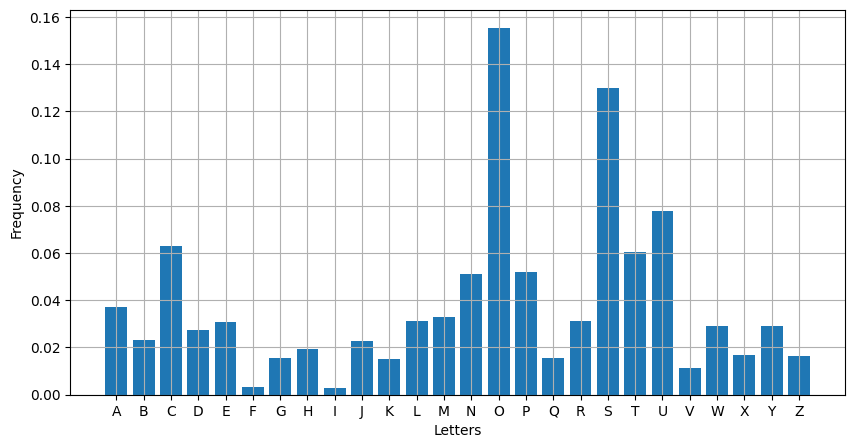
\includegraphics[width=1\linewidth]{images/letters_frequency.png}
    \caption{Frequenza delle lettere nel dataset}
    \label{letters_frequency}
\end{figure}

Come prima operazione è utile aggiungere una colonna iniziale che rappresenti il numero progressivo del dato, in modo da poterlo usare come \texttt{id} del singolo campione e risalire così all'immagine corrispondente. Questo risulta molto utile, ad esempio, quando si vuole individuare uno specifico dato critico che la rete non è riuscita a riconoscere. Questo passaggio è necessario in quanto la prossima trasformazione è la randomizzazione dell'intero dataset. Inizialmente i dati sono ordinati per etichetta dalla A alla Z; utilizzare i dati in questo ordine porterebbe la rete a:
\begin{itemize}
    \item incorrere in overfitting sulle singole lettere anziché imparare pattern generali;
    \item apprendere più lentamente;
    \item avere difficoltà nella ricerca di un minimo globale;
    \item dimenticare le prime lettere apprese.
\end{itemize}
Pertanto, si randomizza prima l'ordine delle righe e successivamente si separano gli indici e le etichette dal dataset vero e proprio.
Oltre a questa suddivisione in colonne, la fase di addestramento richiede anche una suddivisione in righe, con l'obiettivo di ottenere due insiemi di dati: i dati di training, utilizzati per l'addestramento, e i dati di test, utilizzati come controllo sull'andamento dell'errore per evitare overfitting. Una percentuale comune per questo tipo di suddivisione è 80\% di dati training e 20\% dati di test.
Per la rappresentazione del dato e l'elaborazione da parte della rete, anziché un singolo vettore, è necessario disporre i dati secondo una matrice $28\times28$.

Infine, l'output della rete sarà una probabilità, o meglio, un vettore in cui è contenuta la probabilità che il carattere da riconoscere sia quello con l'indice corrispondente alla posizione del dato. Questo tipo di rappresentazione è detta one-hot, il vettore contenente l'etichetta della lettera corrispondente sarà quindi trasformato in un vettore dove ogni elemento è un vettore di zeri con valore 1 all'indice dell'etichetta stessa.
Con i dati organizzati in questo modo è possibile valutare la struttura della rete e le sue componenti.

\begin{lstlisting}[float, language=Python, caption={Codice per la rappresentazione one-hot}]
train_label_OH = np.zeros(shape=(train_label.shape[0], 26))
test_label_OH = np.zeros(shape=(test_label.shape[0], 26))
for idx, n in enumerate(train_label):
    train_label_OH[idx, int(n)] = 1
for idx, n in enumerate(test_label):
    test_label_OH[idx, int(n)] = 1
\end{lstlisting}

\begin{figure}[H]
    \centering
    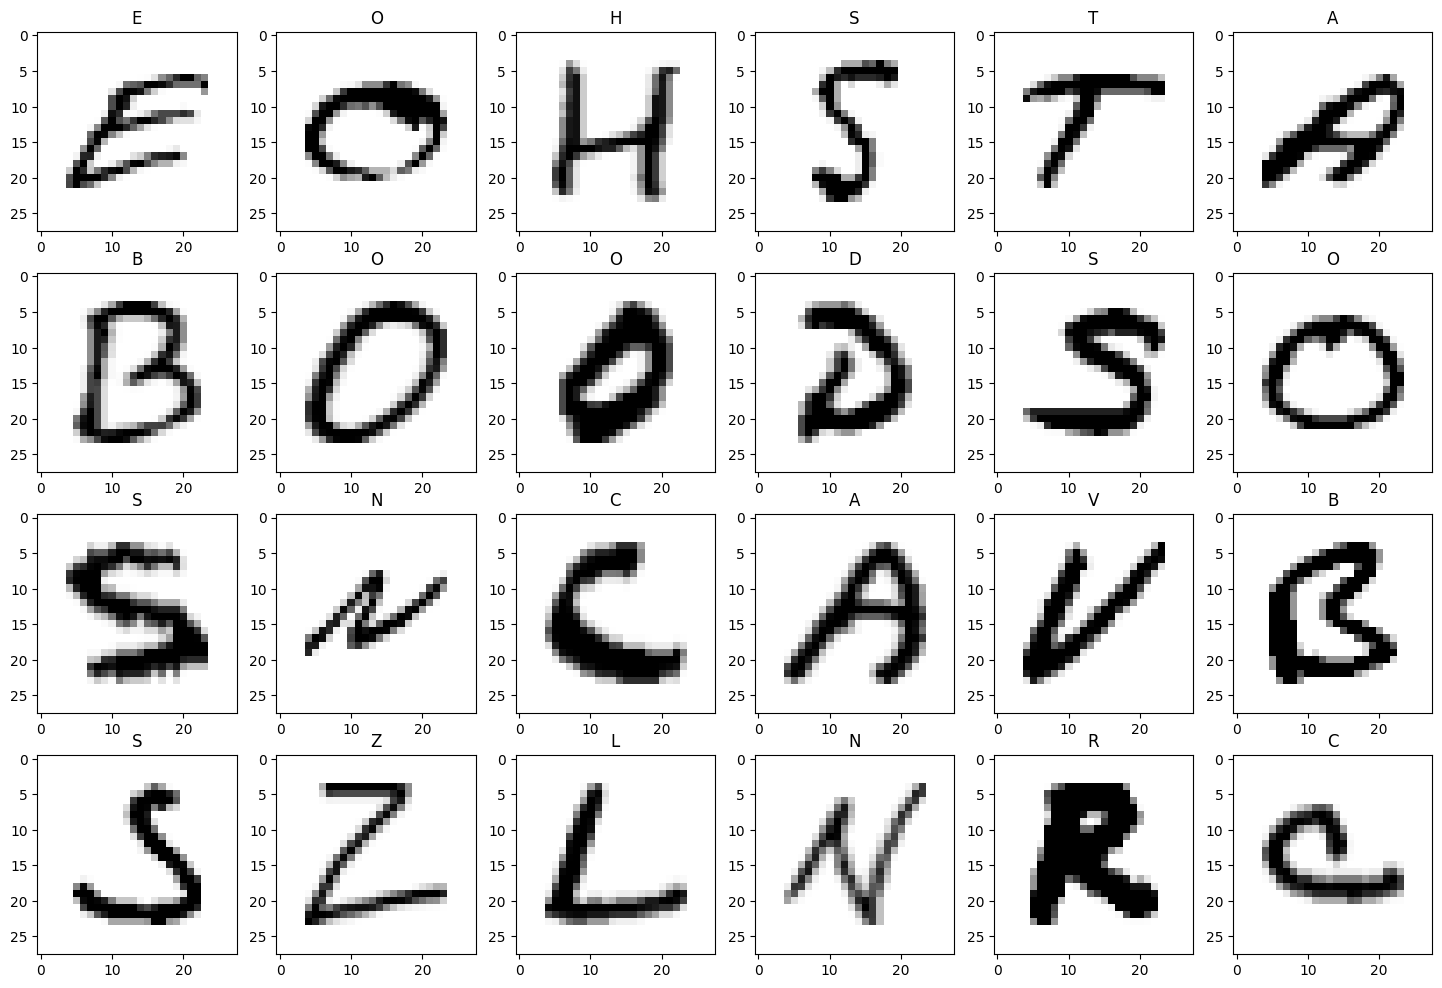
\includegraphics[width=.85\linewidth]{images/some_letters.png}
    \caption{Visualizzazione di alcune lettere}
    \label{some_letters}
\end{figure}

\subsection{Livelli}
Le capacità di una rete neurale dipendono in gran parte dai tipi di livelli che la compongono, così come dal loro ordine e dalla loro interazione.
Nel caso del riconoscimento di immagini, si utilizza una rete convoluzionale (Convolutional Neural Network, CNN), il cui livello principale è quello di convoluzione.
Come già accennato nella sezione \ref{cnn} (\nameref{cnn}), la struttura base di una CNN è costituita dall'alternanza di livelli di convoluzione e livelli di pooling.
Questi livelli rappresentano il fulcro della rete e le conferiscono capacità di "visione", ma non sono sufficienti per costituire una rete completa: i filtri sviluppati estraggono \textit{feature} dalle immagini, che vengono poi elaborate da livelli completamente connessi, i quali calcolano le probabilità associate ai singoli caratteri.
Per fare in modo che gli ultimi strati possano elaborare anch'essi le informazioni, è necessario linearizzare l'output dell'ultimo strato di pooling tramite un livello apposito, quindi passare da una rappresentazione matriciale a una vettoriale.

La struttura della rete è quindi la seguente:
\begin{gather*}
    \text{Input} \\
    \downarrow \\
    \text{Convoluzione} \\
    \downarrow \\
    \text{Pooling} \\
    \downarrow \\
    \text{Convoluzione} \\
    \downarrow \\
    \text{Pooling} \\
    \downarrow \\
    \text{Convoluzione} \\
    \downarrow \\
    \text{Pooling} \\
    \downarrow \\
    \text{Linearizzazione} \\
    \downarrow \\
    \text{Totalmente connesso} \\
    \downarrow \\
    \text{Totalmente connesso} \\
    \downarrow \\
    \text{Totalmente connesso}
\end{gather*}

Anche intuitivamente è facile dire che un solo livello per tipo non sarebbe abbastanza per permettere alla rete di sviluppare le capacità di riconoscimento richieste. Ogni tipo di livello è, quindi, ripetuto tre volte, con convoluzione e pooling alternati e i livelli finali che elaborano le \textit{feature} estratte.

\subsubsection{Covoluzione}
I tre livelli dichiarati nella struttura della rete non sono identici, ma si differenziano per numero di filtri e per ruolo nell'estrazione delle feature, contribuendo in maniera complementare alla capacità di riconoscimento e alla generalizzazione, anche grazie all'azione dei livelli di pooling.

Il primo livello convoluzionale elabora l'input con 32 filtri (kernel) alla piena risoluzione, rilevando pattern locali come bordi, linee e texture semplici.
Il secondo livello, con 64 filtri, opera su un'immagine a risoluzione ridotta a causa del pooling precedente: ciò consente di rilevare combinazioni di \textit{feature} e pattern più complessi, riducendo la dipendenza dalla loro posizione esatta nell'immagine.
Infine, il terzo livello porta il numero di filtri a 128, operando su una rappresentazione ulteriormente ridotta e focalizzandosi su caratteristiche di alto livello, come forme, parti di oggetti o strutture astratte.
Questa progressione è un principio chiave delle reti convoluzionali, poiché consente di mantenere un bilanciamento tra costo computazionale e capacità di rappresentazione.

\subsubsection{Pooling}
Come descritto in precedenza, il pooling è un'operazione che aggrega una regione di pixel in una regione più piccola ed equivale a un'operazione di sottocampionamento. Solitamente le regioni considerate hanno dimensioni $2 \times 2$ e vengono fatte scorrere sull'immagine con stride pari a 2, in modo da valutare ciascun pixel una sola volta. In questo modo, a ogni livello di pooling la risoluzione degli input viene dimezzata.

L'aggregazione delle regioni può avvenire secondo logiche diverse: i 4 pixel possono essere combinati prendendo il valore massimo (max pooling) oppure calcolandone la media (average pooling). I risultati differiscono leggermente: il max pooling tende a enfatizzare le \textit{feature} più marcate e significative, mentre l'average pooling produce rappresentazioni più morbide e diffuse, utili per il riconoscimento di pattern meno netti.
I due approcci possono anche essere combinati per sfruttarne i rispettivi vantaggi: in questo caso può risultare utile utilizzare un metodo nel primo livello di pooling e l'altro nei successivi.

In questo contesto è possibile evidenziare vantaggi e svantaggi dei singoli approcci, ma risulta meno immediato stabilire a livello teorico quale dei metodi garantisca le prestazioni migliori in termini di accuratezza del modello. Per questo è necessario procedere con una valutazione empirica.
I modelli messi a confronto sono quattro:
\begin{itemize}
\item Modello con solo max pooling
\item Modello con solo average pooling
\item Modello con il primo livello di max pooling e i successivi di average pooling
\item Modello con il primo livello di average pooling e i successivi di max pooling
\end{itemize}

\begin{figure}
\centering
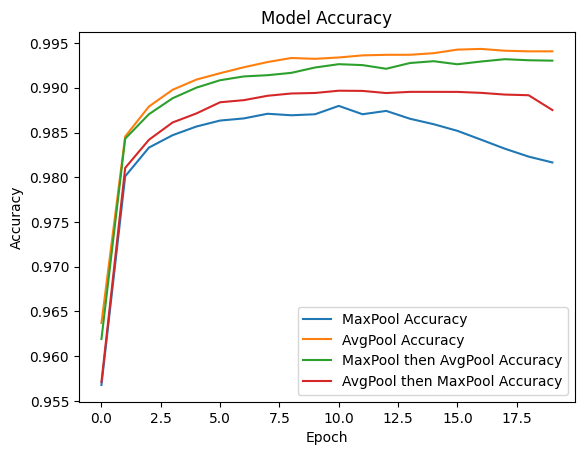
\includegraphics[width=0.7\linewidth]{images/pool_accuracy_comparison.png}
\caption{Confronto di accuratezza tra i metodi di pooling}
\label{pool_accuracy_comparison}
\end{figure}

\begin{figure}
\centering
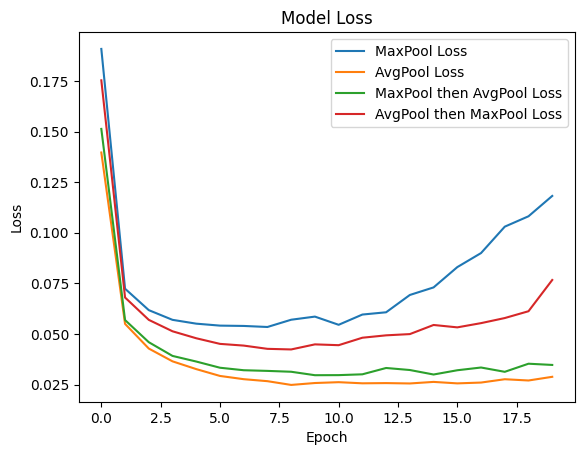
\includegraphics[width=0.7\linewidth]{images/pool_loss_comparison.png}
\caption{Confronto della loss tra i metodi di pooling}
\label{pool_loss_comparison}
\end{figure}

I risultati mostrati in figura \ref{pool_accuracy_comparison} evidenziano come l'average pooling raggiunga un'accuratezza superiore rispetto agli altri metodi, mantenendosi stabile con l'aumentare delle epoche.
Applicare il max pooling al primo livello e l'average pooling ai successivi porta a prestazioni simili, seppur leggermente inferiori, rispetto all'uso esclusivo dell'average pooling. Si può quindi affermare sperimentalmente che l'average pooling abbia un impatto maggiore nei livelli intermedi e finali della rete.
Al contrario, un modello basato esclusivamente su max pooling presenta non solo una perdita (\textit{loss}) più elevata, ma anche una tendenza all'aumento di essa con l'avanzare delle epoche. Questa comparazione permette inoltre di identificare il numero di epoche più adeguato per l'addestramento del modello: si osserva infatti che, oltre la decima epoca, l'accuratezza tende generalmente a diminuire o stabilizzarsi, mentre la \textit{loss} ad aumentare.

È bene precisare che i risultati ottenuti non sono assoluti e sono influenzati da diversi fattori: dipendono, infatti, oltre che dal dataset utilizzato, da come vengono inizializzati i pesi e da come sono distribuiti i dati di training e testing. Nel caso specifico, quindi, si preferisce utilizzare una CNN con livelli di average pool.

\subsection{Funzioni di attivazione}
Le funzioni di attivazione costituiscono una parte fondamentale delle reti neurali, poiché determinano l'uscita di ciascun neurone in base alla combinazione lineare degli ingressi pesati. La loro applicazione introduce non linearità nel modello, consentendo alla rete di apprendere e rappresentare in maniera più efficace relazioni complesse tra dati di input e corrispondenti output, migliorando così la capacità di generalizzazione del sistema.  
Al contrario, l'utilizzo di sole funzioni lineari ridurrebbe la rete a una semplice trasformazione lineare degli input, priva della possibilità di descrivere legami complessi e non linearmente descrivibili.

\subsubsection{ReLU}
La funzione di attivazione \textit{ReLU} (Rectified Linear Unit) è ampiamente utilizzata per la sua semplicità ed efficienza.\\
Essa corrisponde matematicamente alla funzione:
\begin{gather*}
    \text{ReLU}(x) = \max (0, x) \\
    \downarrow \\
    \text{ReLU}(x) =
        \begin{cases}
            0 & \text{ se } \; x\leq 0 \\
            x & \text{ se } \; x > 0 
        \end{cases}
\end{gather*}

ReLU è quindi definita da due funzioni lineari ($y=0$ e $y=x$), rispettivamente per valori negativi e positivi dell'input. Nonostante la sua semplicità, essa introduce non linearità nel modello e permette alla rete di mantenere solo valori positivi, scartando quelli nulli o negativi.  
Nel contesto delle reti convoluzionali, questa proprietà consente di filtrare i pattern non utili al riconoscimento di una specifica caratteristica.  

ReLU viene utilizzata in tutti i livelli convoluzionali e completamente connessi, fatta eccezione per l'ultimo livello che svolge il ruolo di output.

\subsubsection{Softmax}
L'output della rete neurale, che è di classificazione, deve rappresentare una distribuzione di probabilità, così da poter identificare la classe predetta come quella con probabilità più alta. A questo scopo, l'ultimo livello della rete applica comunemente la funzione di attivazione \textit{Softmax}.\\
In termini concettuali, Softmax calcola una frequenza relativa facendo uso della funzione esponenziale:
$$
    \text{Softmax}(x_i) = \frac{\displaystyle e^{\displaystyle x_i}}{\displaystyle \sum_j e^{\displaystyle x_j}}
$$

L'uso della funzione esponenziale consente di:
\begin{itemize}
    \item garantire che la somma delle probabilità sia pari a 1, realizzando una distribuzione valida;
    \item ottenere valori sempre positivi;
    \item amplificare le differenze tra i valori $x_i$, evitando probabilità troppo simili tra loro ed enfatizzando la classe più probabile, rendendo così la decisione più netta.
\end{itemize}

\section{Risultati}
Una rete addestrata come descritto, utilizzando livelli di \textit{average pooling}, raggiunge un'accuratezza del 99.16096\% alla decima epoca, con una \textit{loss} pari a 0.04025.  
Sull'intero insieme di test commette 625 errori su 74490 campioni (0.83904\%) ed è inoltre in grado di riconoscere caratteri disegnati direttamente dall'utente. Attraverso l'utilizzo del mouse, è infatti possibile disegnare un carattere che viene successivamente ridimensionato a una risoluzione di $28 \times 28$ tramite sottocampionamento con interpolazione bilineare e fornito come input alla rete neurale per il riconoscimento.
Grazie all'elevato numero e alla varietà dei dati di addestramento, la rete riesce a riconoscere caratteri scritti con diversi stili, gestendo anche ambiguità con un alto grado di accuratezza.  
Come si osserva in figura \ref{drawn_letters_predicted}, la rete mantiene buone prestazioni anche su lettere decentrate, ambigue o con tratti aperti e non ben definiti.

\begin{figure}[H]
\centering
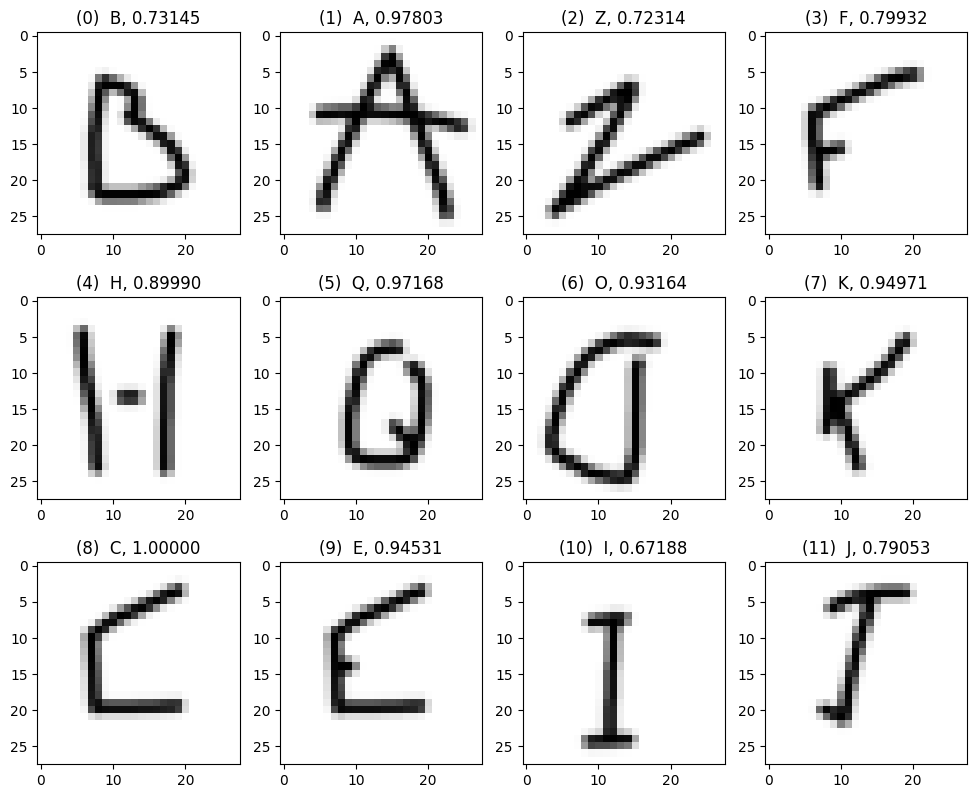
\includegraphics[width=.8\linewidth]{images/drawn_letters_predicted.png}
\caption{Alcune lettere disegnate a mano riconosciute dalla rete neurale}
\label{drawn_letters_predicted}
\end{figure}

\subsection{Step intermedi}
È possibile visualizzare gli step intermedi del riconoscimento effettuato dalla rete, riuscendo a identificare i pattern estratti più importanti e comprendere meglio il "ragionamento" della rete durante il riconoscimento.
Un caso particolare nella figura \ref{drawn_letters_predicted} è quello delle lettere 8 (C) e 9 (E) che hanno la stessa base a differenza del piccolo tratto orizzontale che distingue la C dalla E. Quel piccolo tratto è sufficiente a distinguere le due lettere, quindi durante l'addestramento la rete è riuscita a definire una buona scelta di estrazione di \textit{feature} per determinare la differenza tra i due caratteri.

\begin{figure}[H]
\centering
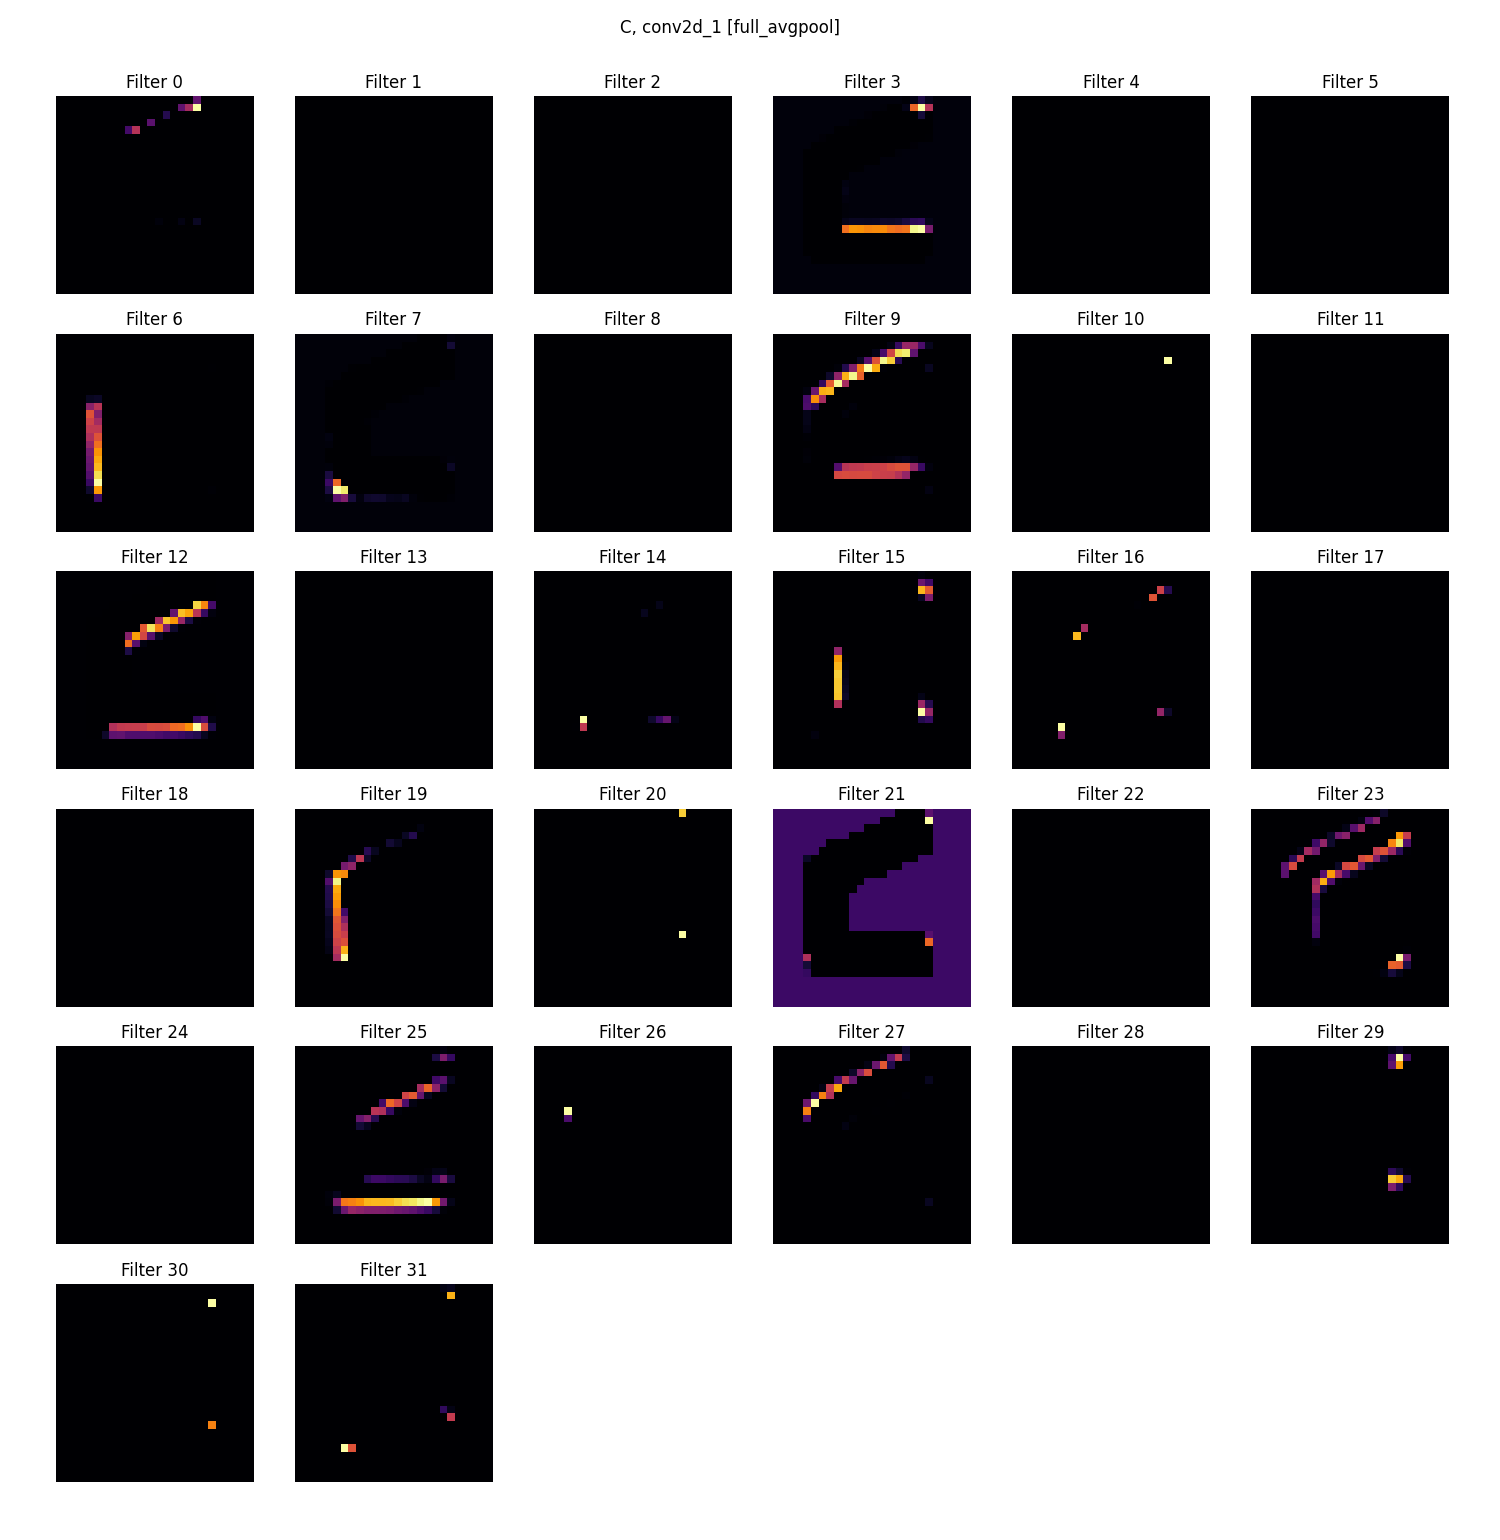
\includegraphics[width=1\linewidth]{images/C_full_avgpool_layer_0.png}
\caption{Risultati dei filtri applicati dal primo layer di convoluzione alla lettera C}
\label{first_layer_filters_C}
\end{figure}

\begin{figure}[H]
\centering
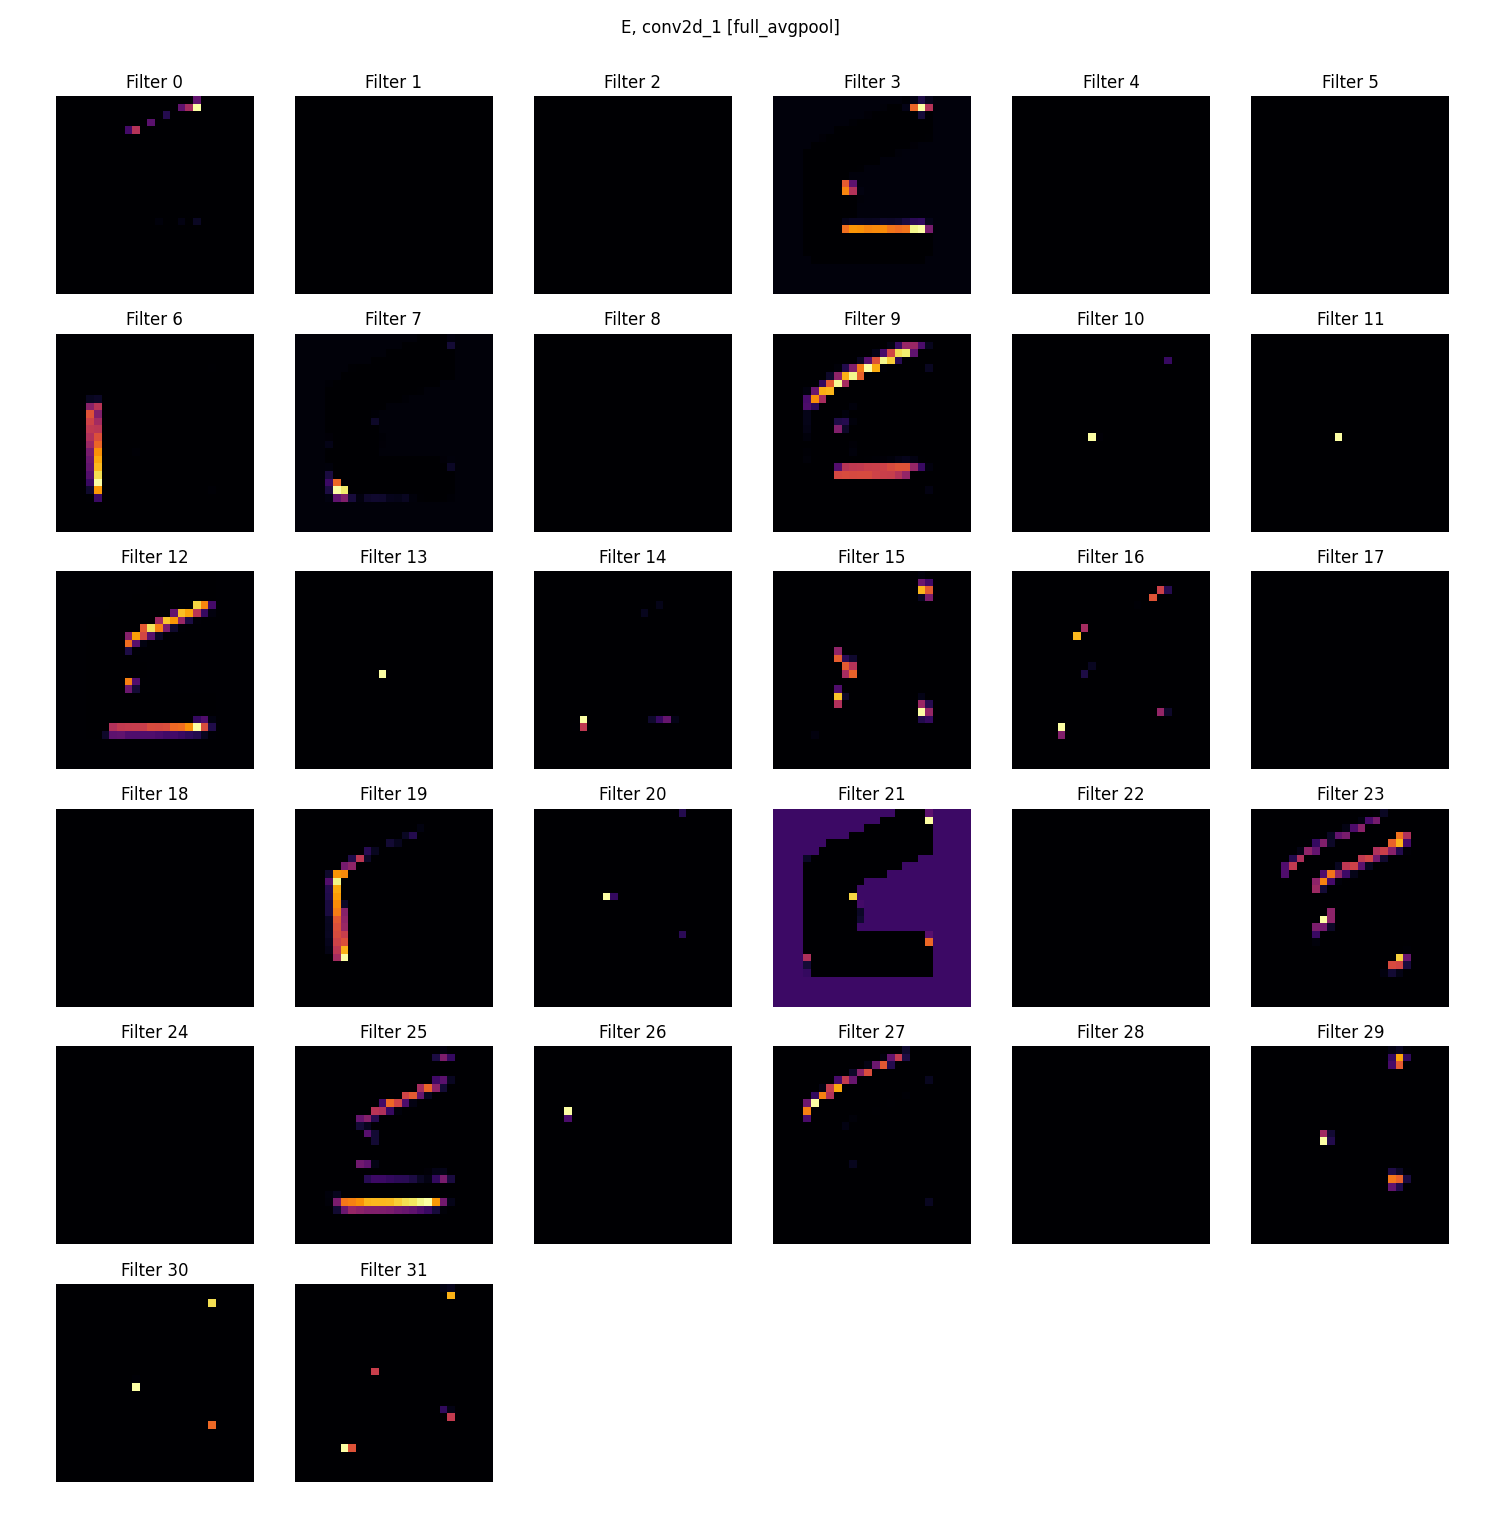
\includegraphics[width=1\linewidth]{images/E_full_avgpool_layer_0.png}
\caption{Risultati dei filtri applicati dal primo layer di convoluzione alla lettera E}
\label{first_layer_filters_E}
\end{figure}

Nelle figure \ref{first_layer_filters_C} e \ref{first_layer_filters_E} è possibile visualizzare i risultati delle applicazioni dei filtri che vengono usati nel primo livello di convoluzione. Come è possibile notare, anche se la differenza tra i due disegni è minima (approssimativamente la differenza è in una regione di $3 \times 3$ pixel), molti filtri estraggono quel tratto orizzontale rendendolo molto visibile e determinante per la scelta del carattere più probabile. Alcuni di questi filtri sono il numero 3, 12, 15 e 23 che evidenziano il tratto in discussione.
Nei livelli successivi, con l'aumento del numero di filtri, le \textit{feature} vengono ulteriormente elaborate e combinate per raffinare il processo di riconoscimento.  
Questi risultati intermedi mostrano anche come la rete riesca a individuare pattern orizzontali (es. filtri 3 e 25), verticali (es. 6, 15 e 19) e diagonali (es. 23 e 27), in linea con quanto discusso nei capitoli precedenti. Tali \textit{feature} contribuiscono a scomporre l'informazione visiva in elementi essenziali che, combinati, consentono il riconoscimento del carattere.

\begin{figure}[H]
\centering
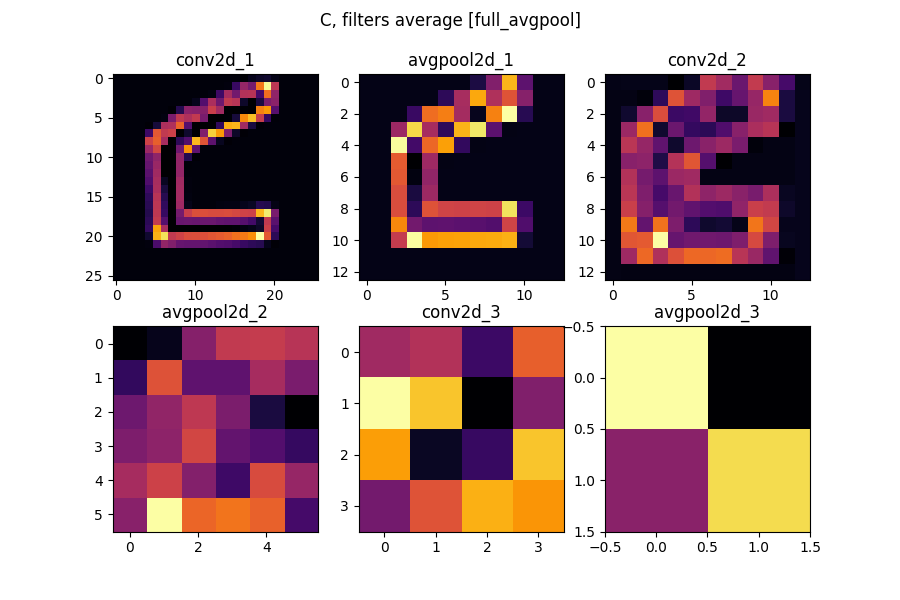
\includegraphics[width=.6\linewidth]{images/C_full_avgpool_filters_avg.png}
\caption{Media dei risultati dei filtri applicati dai layer alla lettera C}
\label{avg_filters_C}
\end{figure}

\begin{figure}[H]
\centering
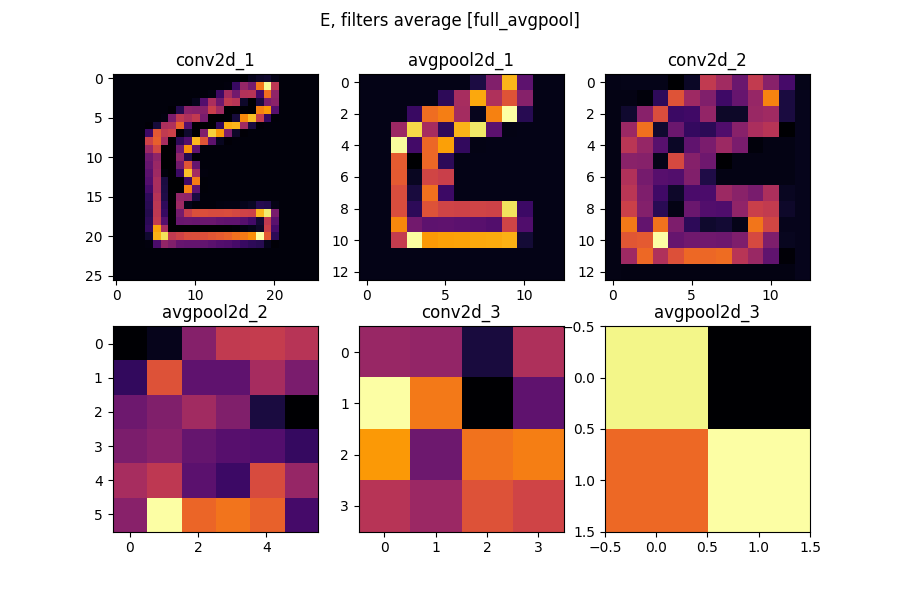
\includegraphics[width=.6\linewidth]{images/E_full_avgpool_filters_avg.png}
\caption{Media dei risultati dei filtri applicati dai layer alla lettera E}
\label{avg_filters_E}
\end{figure}

Un'ulteriore rappresentazione utile è data dalla media dei risultati dei vari filtri per ogni livello, come si può vedere nelle figure \ref{avg_filters_C} e \ref{avg_filters_E}. I grafici offrono un'idea visiva di come si concentrano i filtri nei vari livelli e di come il pooling agisce sui risultati di convoluzione.
Soprattutto nei primi livelli è evidente come la rete si focalizzi sui contorni della lettera per determinarne la forma, mentre dopo il secondo layer di convoluzione la visualizzazione perde di significato in quanto i filtri aumentano esponenzalmente di numero e la risoluzione diminuisce, ma è comunque interessante notare come la piccola differenza nel tratto orizzontale negli input porti a una grande differenza nell'ultimo layer.
È bene ribadire che queste ultime figure non sono pienamente rappresentative, poiché i filtri hanno un significato in quanto pesati individualmente, non come media, tuttavia è comunque un utile strumento di intuizione visiva di come l'informazione viene elaborata lungo la rete.

\subsection{Limiti}

%TODO ricorda di parlare di quanto siano poche le 'I', porta a riconoscerle spesso come 'T'

\end{document}